In this section, we describe our experimental study of the method proposed in the paper.
Four settings were used to account for the three variants of the barrier forming, the instances and solution examples of which are shown in ~\ref{fig:bf-exp}. 
The experiments were carried out on a Hexa-Core processor with 16 GiB memory, and Gurobi
\cite{optimization2019gurobi} was used as the Integer Programming solver.
In the polygonal object instances generation, random polygons were generated by computing traveling salesperson tour (TSP) tours of random point sets each consisting of $3$ to $6$ vertices, which we found to be effective in generating sensible looking polygons that are not necessarily convex.
%
When a problem setup contains obstacles, the number of obstacles in the environment is set to be the same as the number of objects for each object set.


\begin{figure*}[ht]
    \centering
    
    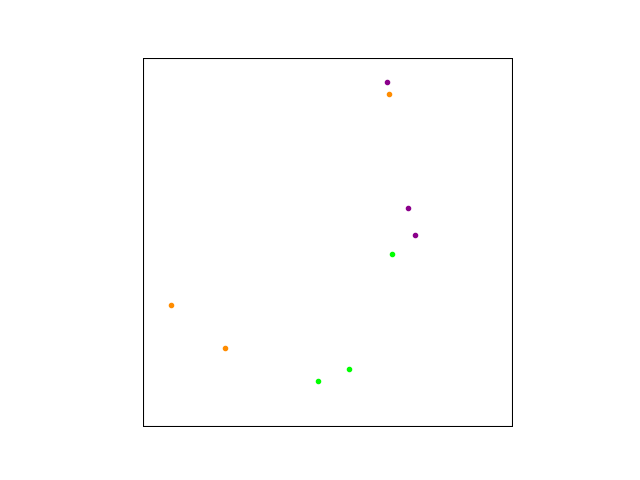
\includegraphics[trim=80 20 80 20,clip, width = .24\textwidth]{chapters/bf/fig/exp_1_instance.png}
    \hspace{-.1in}
    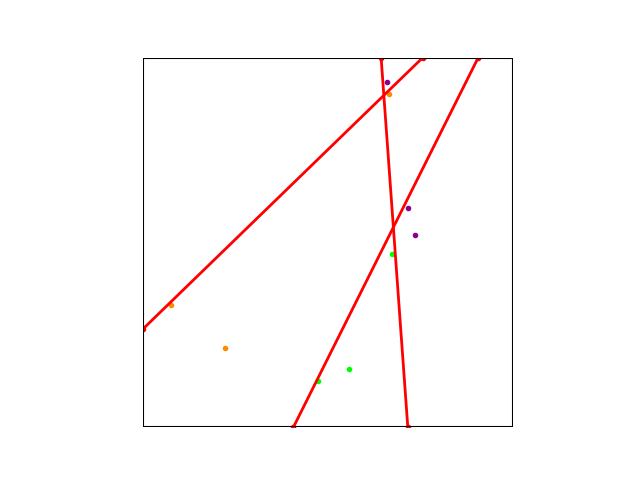
\includegraphics[trim=80 20 80 20,clip, width = .24\textwidth]{chapters/bf/fig/exp_1_result.png}
    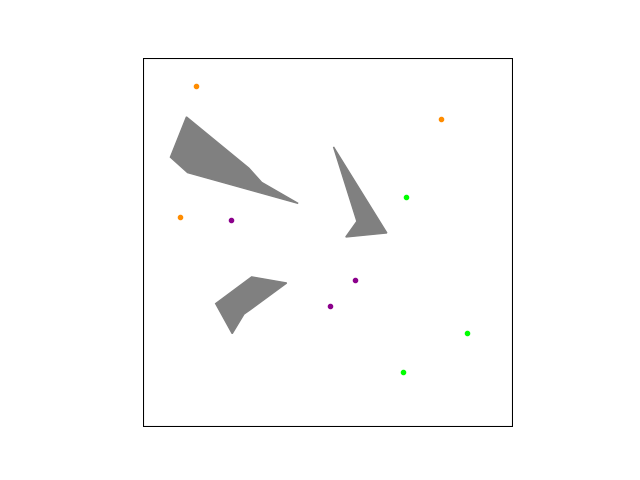
\includegraphics[trim=80 20 80 20,clip, width = .24\textwidth]{chapters/bf/fig/exp_2_instance.png}
    \hspace{-.1in}
    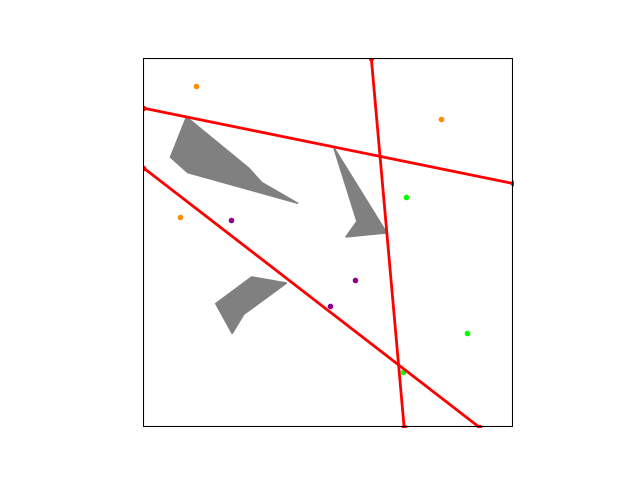
\includegraphics[trim=80 20 80 20,clip, width = .24\textwidth]{chapters/bf/fig/exp_2_result.png}
    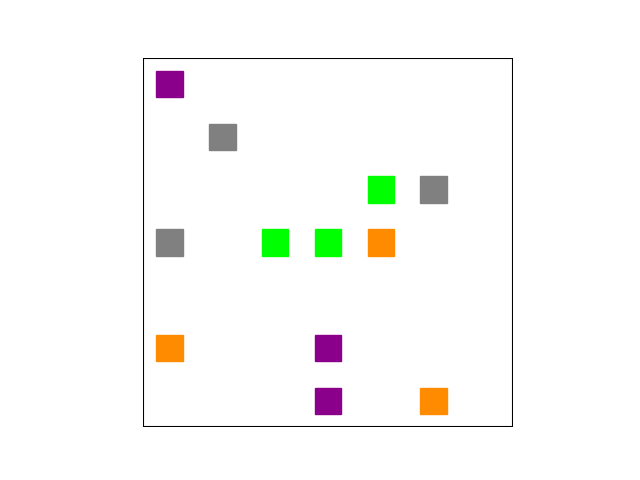
\includegraphics[trim=80 20 80 20,clip, width = .24\textwidth]{chapters/bf/fig/exp_3_instance.png}
    \hspace{-.1in}
    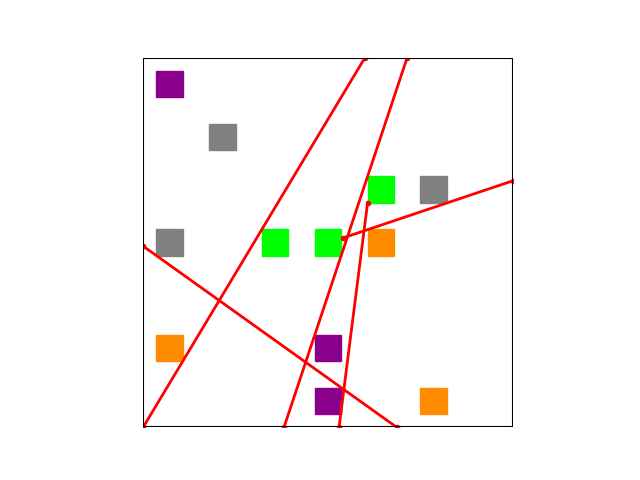
\includegraphics[trim=80 20 80 20,clip, width = .24\textwidth]{chapters/bf/fig/exp_3_result.png}
    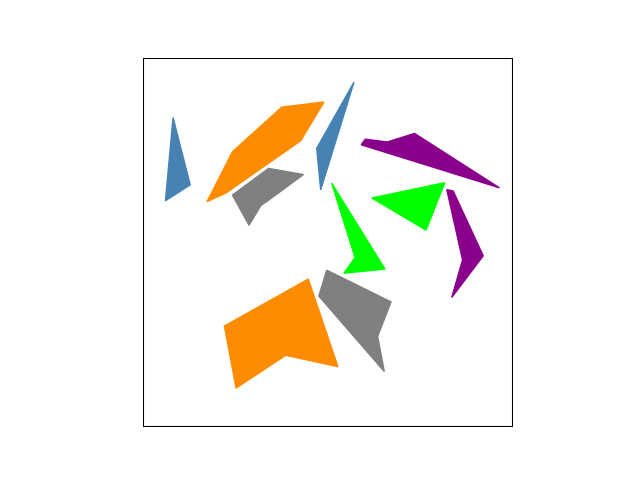
\includegraphics[trim=80 20 80 20,clip, width = .24\textwidth]{chapters/bf/fig/exp_4_instance.png}
    \hspace{-.1in}
    % 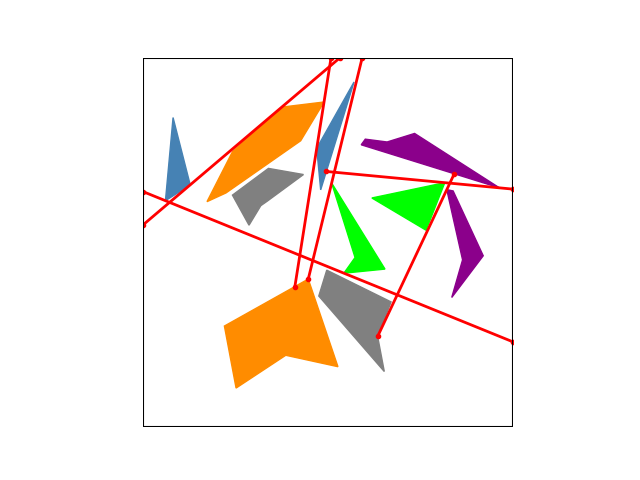
\includegraphics[trim=80 20 80 20,clip, width = .24\textwidth]{fig/exp_4_result.png}
    \begin{overpic}[trim=80 20 80 20,clip, width = .24\textwidth]{chapters/bf/fig/exp_4_result.png}
    \put(-202, 98) {(a)}
    \put(-3, 98) {(b)}
    \put(-202, 0) {(c)}
    \put(-3, 0) {(d)}
    
    \end{overpic}
    \caption{Illustration of the four types of instances used in our  experimental evaluation. (a) Barrier forming for point sets. (b) Barrier forming to separate point sets from polygonal obstacles. (c) Barrier forming to separate uniform square-shaped objects among uniform square-shaped obstacles. (d) Barrier forming to separate random polygonal objects among random polygonal obstacles.}
    \label{fig:bf-exp}
\end{figure*}

\subsection{Separating Sets of Points}
The first type of instances aims at forming barriers among randomly generated point sets, 
shown in ~\ref{fig:bf-exp}(a). The number of object sets to separate from each other range from $2$ to $4$, 
and the number of objects in each set range from $1$ to $6$. 
Each entry in the Table ~\ref{tab:bf-expr_1} is the result of average computation times over 10 instances. From the result, we observe that the IP based method is fairly effective in separating two sets of objects with the presence of obstacles. The method scales to about $10$ point objects plus obstacles. The number of line segments in the optimal barrier are generally small, e.g., $3$-$10$.

\begin{table}[ht]
    \centering
    \begin{tabular}{|c|c|c|c|c|c|c|}\hline
        %  \diagbox{\#Set}{\#Objects}
        \#Sets &  1 & 2 & 3 & 4& 5& 6\\\hline
 2& 0.005 & 0.011 & 0.083 & 0.419 & 2.010 & 15.887 \\\hline
 3& 0.013 & 0.316 & 12.773 & 962.883 & - & - \\\hline
 4& 0.051 & 14.641 &  -& - &  -&- \\\hline
\end{tabular}
    \caption{Running time in seconds for Expr. 1 where all objects and obstacles are points (~\ref{fig:bf-exp}(a)). ``-'' denotes the result cannot be computed in 1h on average (the same is true for other tables). 
    The column index means the number of objects in each set, and the row index means the number of object sets.
    The number of obstacles is set to be the same as the number of objects for each set. These also apply to the following tables.
    }
    \label{tab:bf-expr_1}
\end{table}

 The second type of instances generates barriers for randomly generated 
 point sets with the existence of polygonal obstacles, shown in ~\ref{fig:bf-exp}(b). 
 The other specification is the same as Expr. 1, and the number of obstacles for each experiment is set to be the same as the number of objects for each set. 
 The resulting time cost, shown in Table~\ref{tab:bf-expr_2}, is similar to Expr. 1 despite the existence of obstacles.
 %
 Similarly, we observe decent performance when it comes to separating two sets of objects among obstacles. 
 %
 The introduction of polygonal obstacles does not cause performance degradation. 


\begin{table}[ht]
    \centering
    \begin{tabular}{|c|c|c|c|c|c|c|}\hline
        %  \diagbox{\#Set}{\#Objects}
        \#Set &  1 & 2 & 3 & 4& 5& 6\\\hline
2& 0.009 & 0.061 & 0.480 & 5.899 & 3.433 & 21.121\\\hline
 3& 0.044 & 3.287 & 71.346 & 320.955 & - & -\\\hline
 4& 0.249 & 13.801 & - & - & - & -\\\hline
    \end{tabular}
    \caption{Running time in seconds for Expr. 2 where objects to be separated are points and obstacles are randomly generated polygons (~\ref{fig:bf-exp}(b)). 
    }
    \label{tab:bf-expr_2}
    \vspace{-2mm}
\end{table}
 
\subsection{Separating Sets of Polygonal Shapes}
The third set of experiments uses randomly placed squares as obstacles and objects, shown in ~\ref{fig:bf-exp}(c). The squares are sampled from a $7\times7$ grid. Each square is half the scale of a grid cell and is positioned at the center of a grid cell. The running time for this case turns out to be the greatest among all $4$ experiments. This is due to the rectlinear nature of the instance, which creates many small cells that are difficult to process. 

\begin{table}[ht]
    \centering
    \begin{tabular}{|c|c|c|c|c|c|c|}\hline
        %  \diagbox{\#Set}{\#Objects}
         \#Set &  1 & 2 & 3 & 4& 5& 6\\\hline
 2 & 0.010 & 0.065 & 0.652 & 31.536 & 575.933 & 1259.653\\\hline
 3 & 0.065 & 10.608 & 337.050 & - & - & -\\\hline
 4 & 0.235 & 124.963 & - & - & - & -\\\hline
    \end{tabular}
    \caption{Running time in seconds for Expr. 3 with square-shaped objects and obstacles (~\ref{fig:bf-exp}(c)). ``-'' denotes the result cannot be computed in 1h on average. 
    % The number of obstacles is set to be the same as the number of objects for each set.
    }
    \label{tab:bf-expr_3}
    \vspace{-2mm}
\end{table}
 
The last type of instances uses random polygons with $3\sim 6$ vertices
as objects and obstacles, shown in ~\ref{fig:bf-exp}(d). 
Counter intuitively, these experiments turn out to have the least time cost among the $4$ experiments despite the most complex environment; we see that even for four different sets of objects where each set contains six objects, the problem can be solved very quickly. %This is due to the larger area of the object sets, which limits the choices of barrier line segments. 

In the end, the running time of the algorithm provided is more dependent on the number of cells and candidate barrier line segments. 
When objects and obstacles are more densely packed in the experiment, 
there will be less barrier candidates and cells due to collisions between objects and the candidate line segments.
While in a sparse environment or even with just point objects, there will be more barrier candidates and cells.
This explains the reduced time cost in a more complex environment from the sparse settings.

\begin{table}[ht]
    \centering
    \begin{tabular}{|c|c|c|c|c|c|c|}\hline
        %  \diagbox{\#Set}{\#Objects}
         \#Set&  1 & 2 & 3 & 4& 5& 6\\\hline
2& 0.006 & 0.031 & 0.080 & 0.143 & 0.157 & 0.156 \\\hline
3& 0.031 & 0.234 & 0.994 & 1.271 & 1.980 & 1.187 \\\hline
4& 0.103 & 0.518 & 3.000 & 6.050 & 9.692 & 17.996 \\\hline 
    \end{tabular}
    \caption{Running time in seconds for Expr. 4 where both the objects to be separated and the obstacles are randomly generated polygons 
    (~\ref{fig:bf-exp}(d)).
    % The number of obstacles is set to be the same as the number of objects for each set.
    }
    \label{tab:bf-expr_4}
    \vspace{-2mm}
\end{table}